\chapter{Results and Discussion}

\section{Back-splice junction (BSJ) detection}

- Five different BSJ detection tools were used
- Basic upset plot
- Ignoring strand information
- Analysis of allowed mismatch distances

\begin{figure}[ht]
    \begin{tabular}{cc}
        \begin{subfigure}{.5\textwidth}
            \centering

            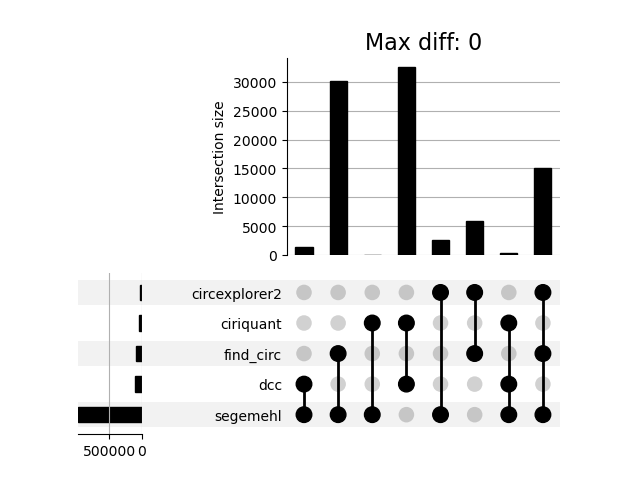
\includegraphics[width=.8\linewidth]{chapters/4_results_and_discussion/figures/detection/min_samples_0/upset/diff_0.png}
            \caption{1:1 match}
            \label{fig:detection_upset_full}
        \end{subfigure}
         &
        \begin{subfigure}{.5\textwidth}
            \centering

            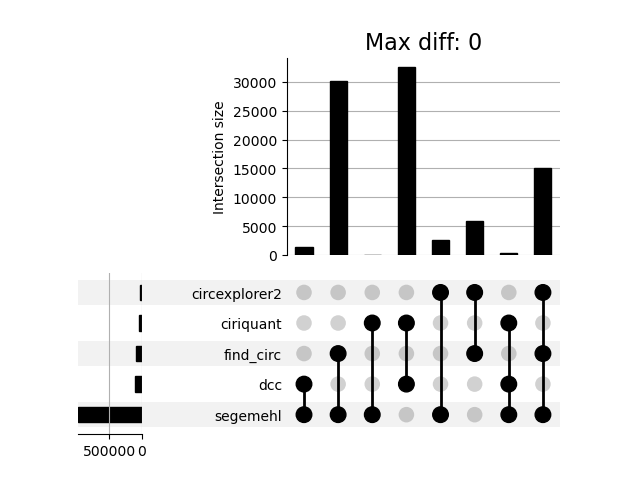
\includegraphics[width=.8\linewidth]{chapters/4_results_and_discussion/figures/detection/min_samples_0/upset/diff_0.png}
            \caption{Ignoring strand}
            \label{fig:detection_upset_nostrand}
        \end{subfigure} \\
        \multicolumn{2}{c}{
            \begin{subfigure}{\textwidth}
                \centering

                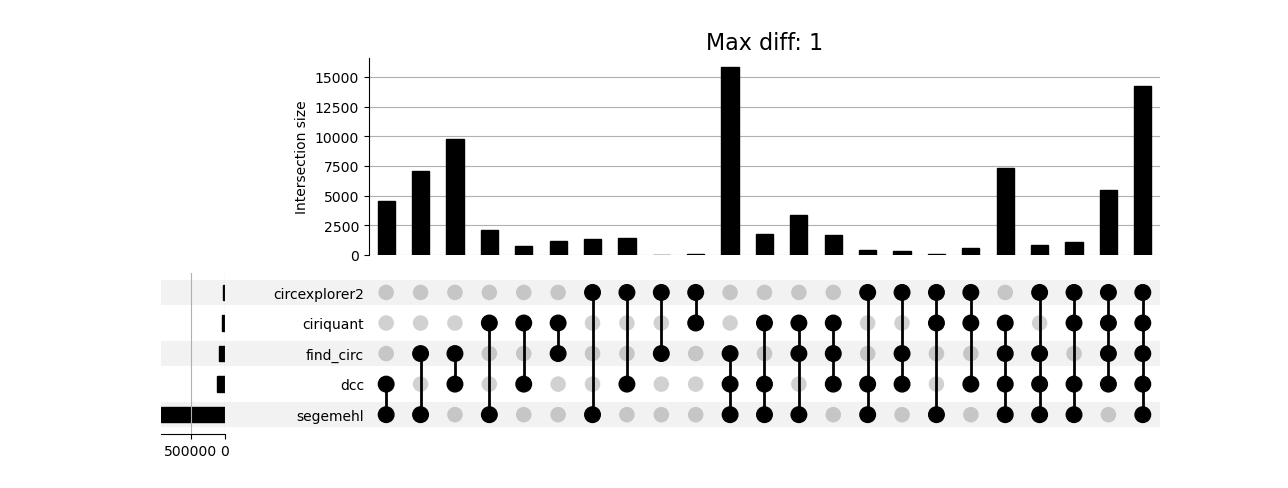
\includegraphics[width=.8\linewidth]{chapters/4_results_and_discussion/figures/detection/min_samples_0/upset/diff_1.png}
                \caption{Microshift}
                \label{fig:detection_upset_microshift}

            \end{subfigure}}
    \end{tabular}
    \caption{Upset plots} % TODO: Add detailed caption
    \label{fig:detection_upset}
\end{figure}

\begin{figure}[ht]
    \begin{tabular}{cc}
        \begin{subfigure}{.5\textwidth}
            \centering

            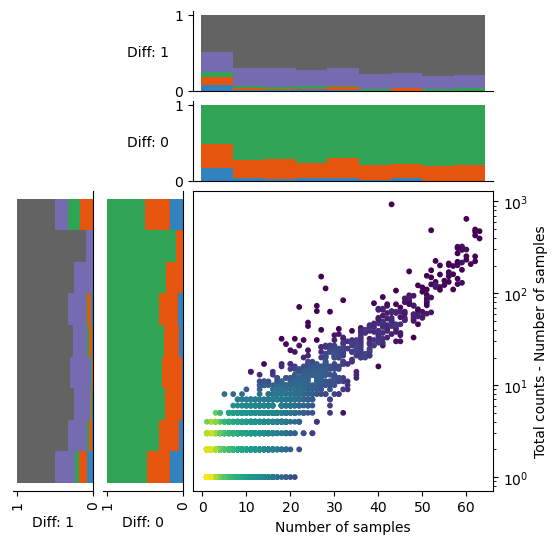
\includegraphics[width=.8\linewidth]{chapters/4_results_and_discussion/figures/detection/min_samples_0/density/circexplorer2.png}
            \caption{CircExplorer2}
            \label{fig:detection_density_circexplorer2}
        \end{subfigure}
         &
        \begin{subfigure}{.5\textwidth}
            \centering

            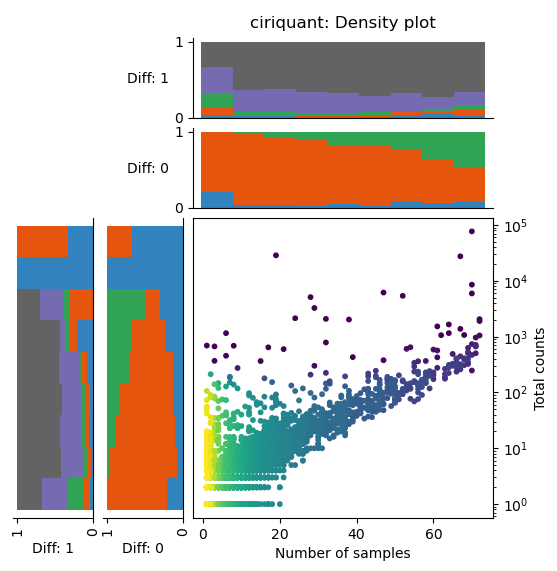
\includegraphics[width=.8\linewidth]{chapters/4_results_and_discussion/figures/detection/min_samples_0/density/ciriquant.png}
            \caption{CiriQuant}
            \label{fig:detection_density_ciriquant}
        \end{subfigure} \\
        \begin{subfigure}{.5\textwidth}
            \centering

            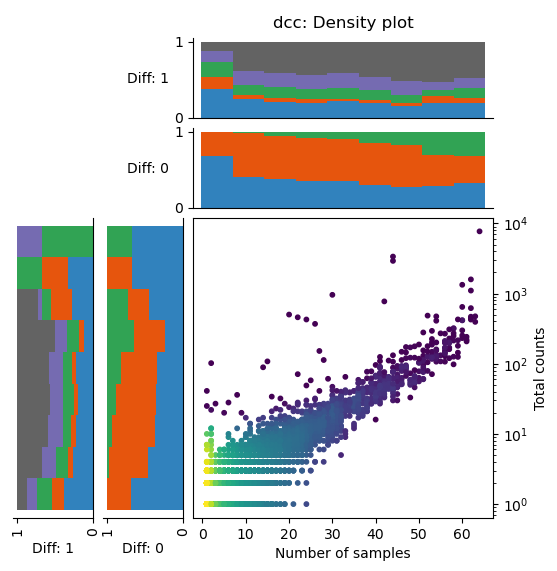
\includegraphics[width=.8\linewidth]{chapters/4_results_and_discussion/figures/detection/min_samples_0/density/dcc.png}
            \caption{DCC}
            \label{fig:detection_density_dcc}
        \end{subfigure}
         &
        \begin{subfigure}{.5\textwidth}
            \centering

            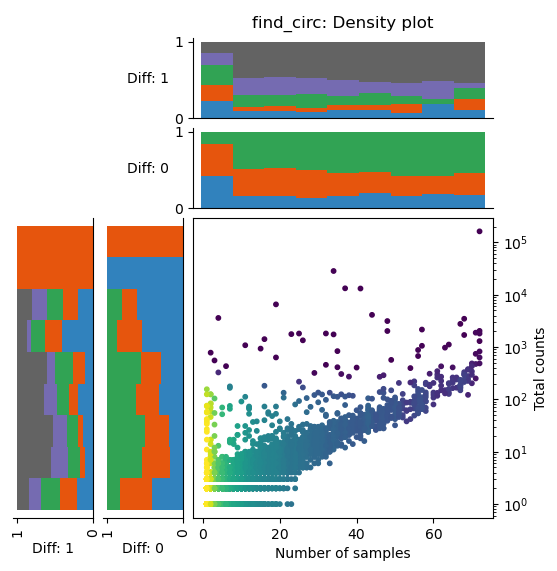
\includegraphics[width=.8\linewidth]{chapters/4_results_and_discussion/figures/detection/min_samples_0/density/find_circ.png}
            \caption{find\_circ}
            \label{fig:detection_density_find-circ}
        \end{subfigure}
    \end{tabular}
    \caption{Density plots} % TODO: Add detailed caption
    \label{fig:detection_density}
\end{figure}

\section{Quantification}

\section{Differential expression analysis}

\section{Biological interpretation}
